\documentclass[a4paper,12pt,twoside]{memoir}
\usepackage{longtable}
\usepackage{btp}    % Use the trainermanual package option (i.e. \usepackage[trainermanual]{btp}) to generate the Trainer's version of the manual
%\usepackage[
%  noinfo,
%  cam,
%  cross,                % crosses as marks
%  a4,
%  width=6.25in,         % the width of the galley
%  height=9.25in,        % the height of the galley
%  center                % actual page is centered on the galley
%]{crop}

\usepackage{tikz}
\usetikzlibrary{shapes,arrows}

% Set some Workshop specific info
\setWorkshopTitle{Introduction To NGS Data \\ [3mm]
\& Analytic Tools}
\setWorkshopVenue{Bioinformatics Hub\newline
University of Adelaide}
\setWorkshopDate{\today}
\setWorkshopAuthor{
Steve Pederson
}

\begin{document}

%
% Workshop Title Page
%
\workshoptitlepage

%
% CC-BY
%
\input{licences/licence.tex}
\clearpage

\tableofcontents

\chapter{Workshop Information}
\clearpage

%
% Trainers Page
%
\section{The Trainers}

\newlength{\trainerIconWidth}
\setlength{\trainerIconWidth}{2.0cm}

\begin{center}
\begin{longtable}{>{\centering\arraybackslash} m{1.1\trainerIconWidth} m{1\textwidth}}

  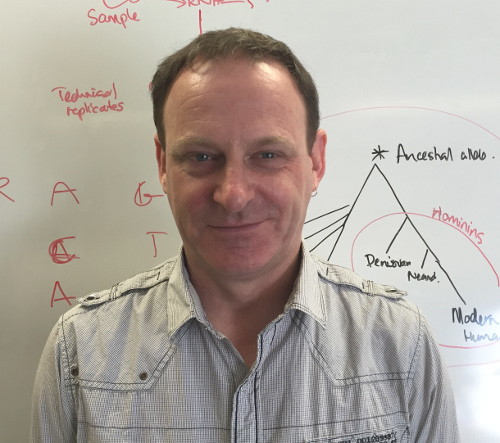
\includegraphics[width=\trainerIconWidth]{photos/steveped.jpeg} &
    \textbf{Mr. Steve Pederson}\newline
    Co-ordinator\newline
    Bioinformatics Hub\newline
    The University of Adelaide\newline
    South Australia\newline
    \mailto{stephen.pederson@adelaide.edu.au}\\
     \\
     
  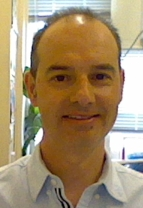
\includegraphics[width=\trainerIconWidth]{photos/Terry.jpg} &
    \textbf{Dr. Terry Bertozzi}\newline
    Bioinformatician\newline
    SA Museum\newline
    South Australia\newline
    \mailto{ Terry.Bertozzi@samuseum.sa.gov.au}\\
     \\
    
  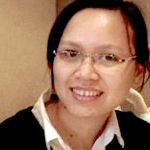
\includegraphics[width=\trainerIconWidth]{photos/hien.png} &
    \textbf{Dr. Hien To}\newline
    Bioinformatician\newline
    Bioinformatics Hub\newline
    The University of Adelaide\newline
    South Australia\newline
    \mailto{hien.to@adelaide.edu.au}\\
   \\
    
  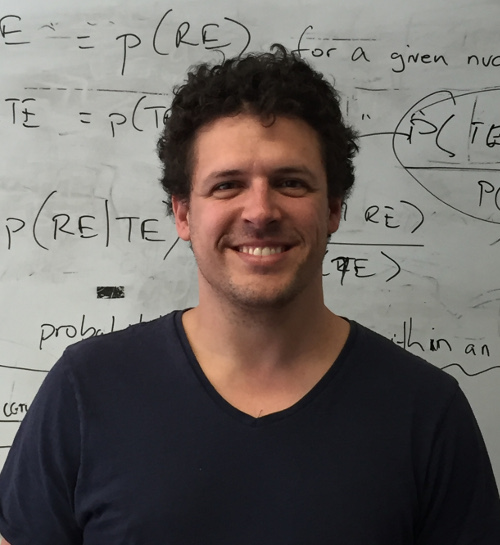
\includegraphics[width=\trainerIconWidth]{photos/jimmyb.jpg} &
    \textbf{Dr. Jimmy Breen}\newline
    Bioinformatician\newline
    Bioinformatics Hub \& Robinson Research Institure\newline
    The University of Adelaide\newline
    South Australia\newline
    \mailto{jimmy.breen@adelaide.edu.au}\\
    \\

  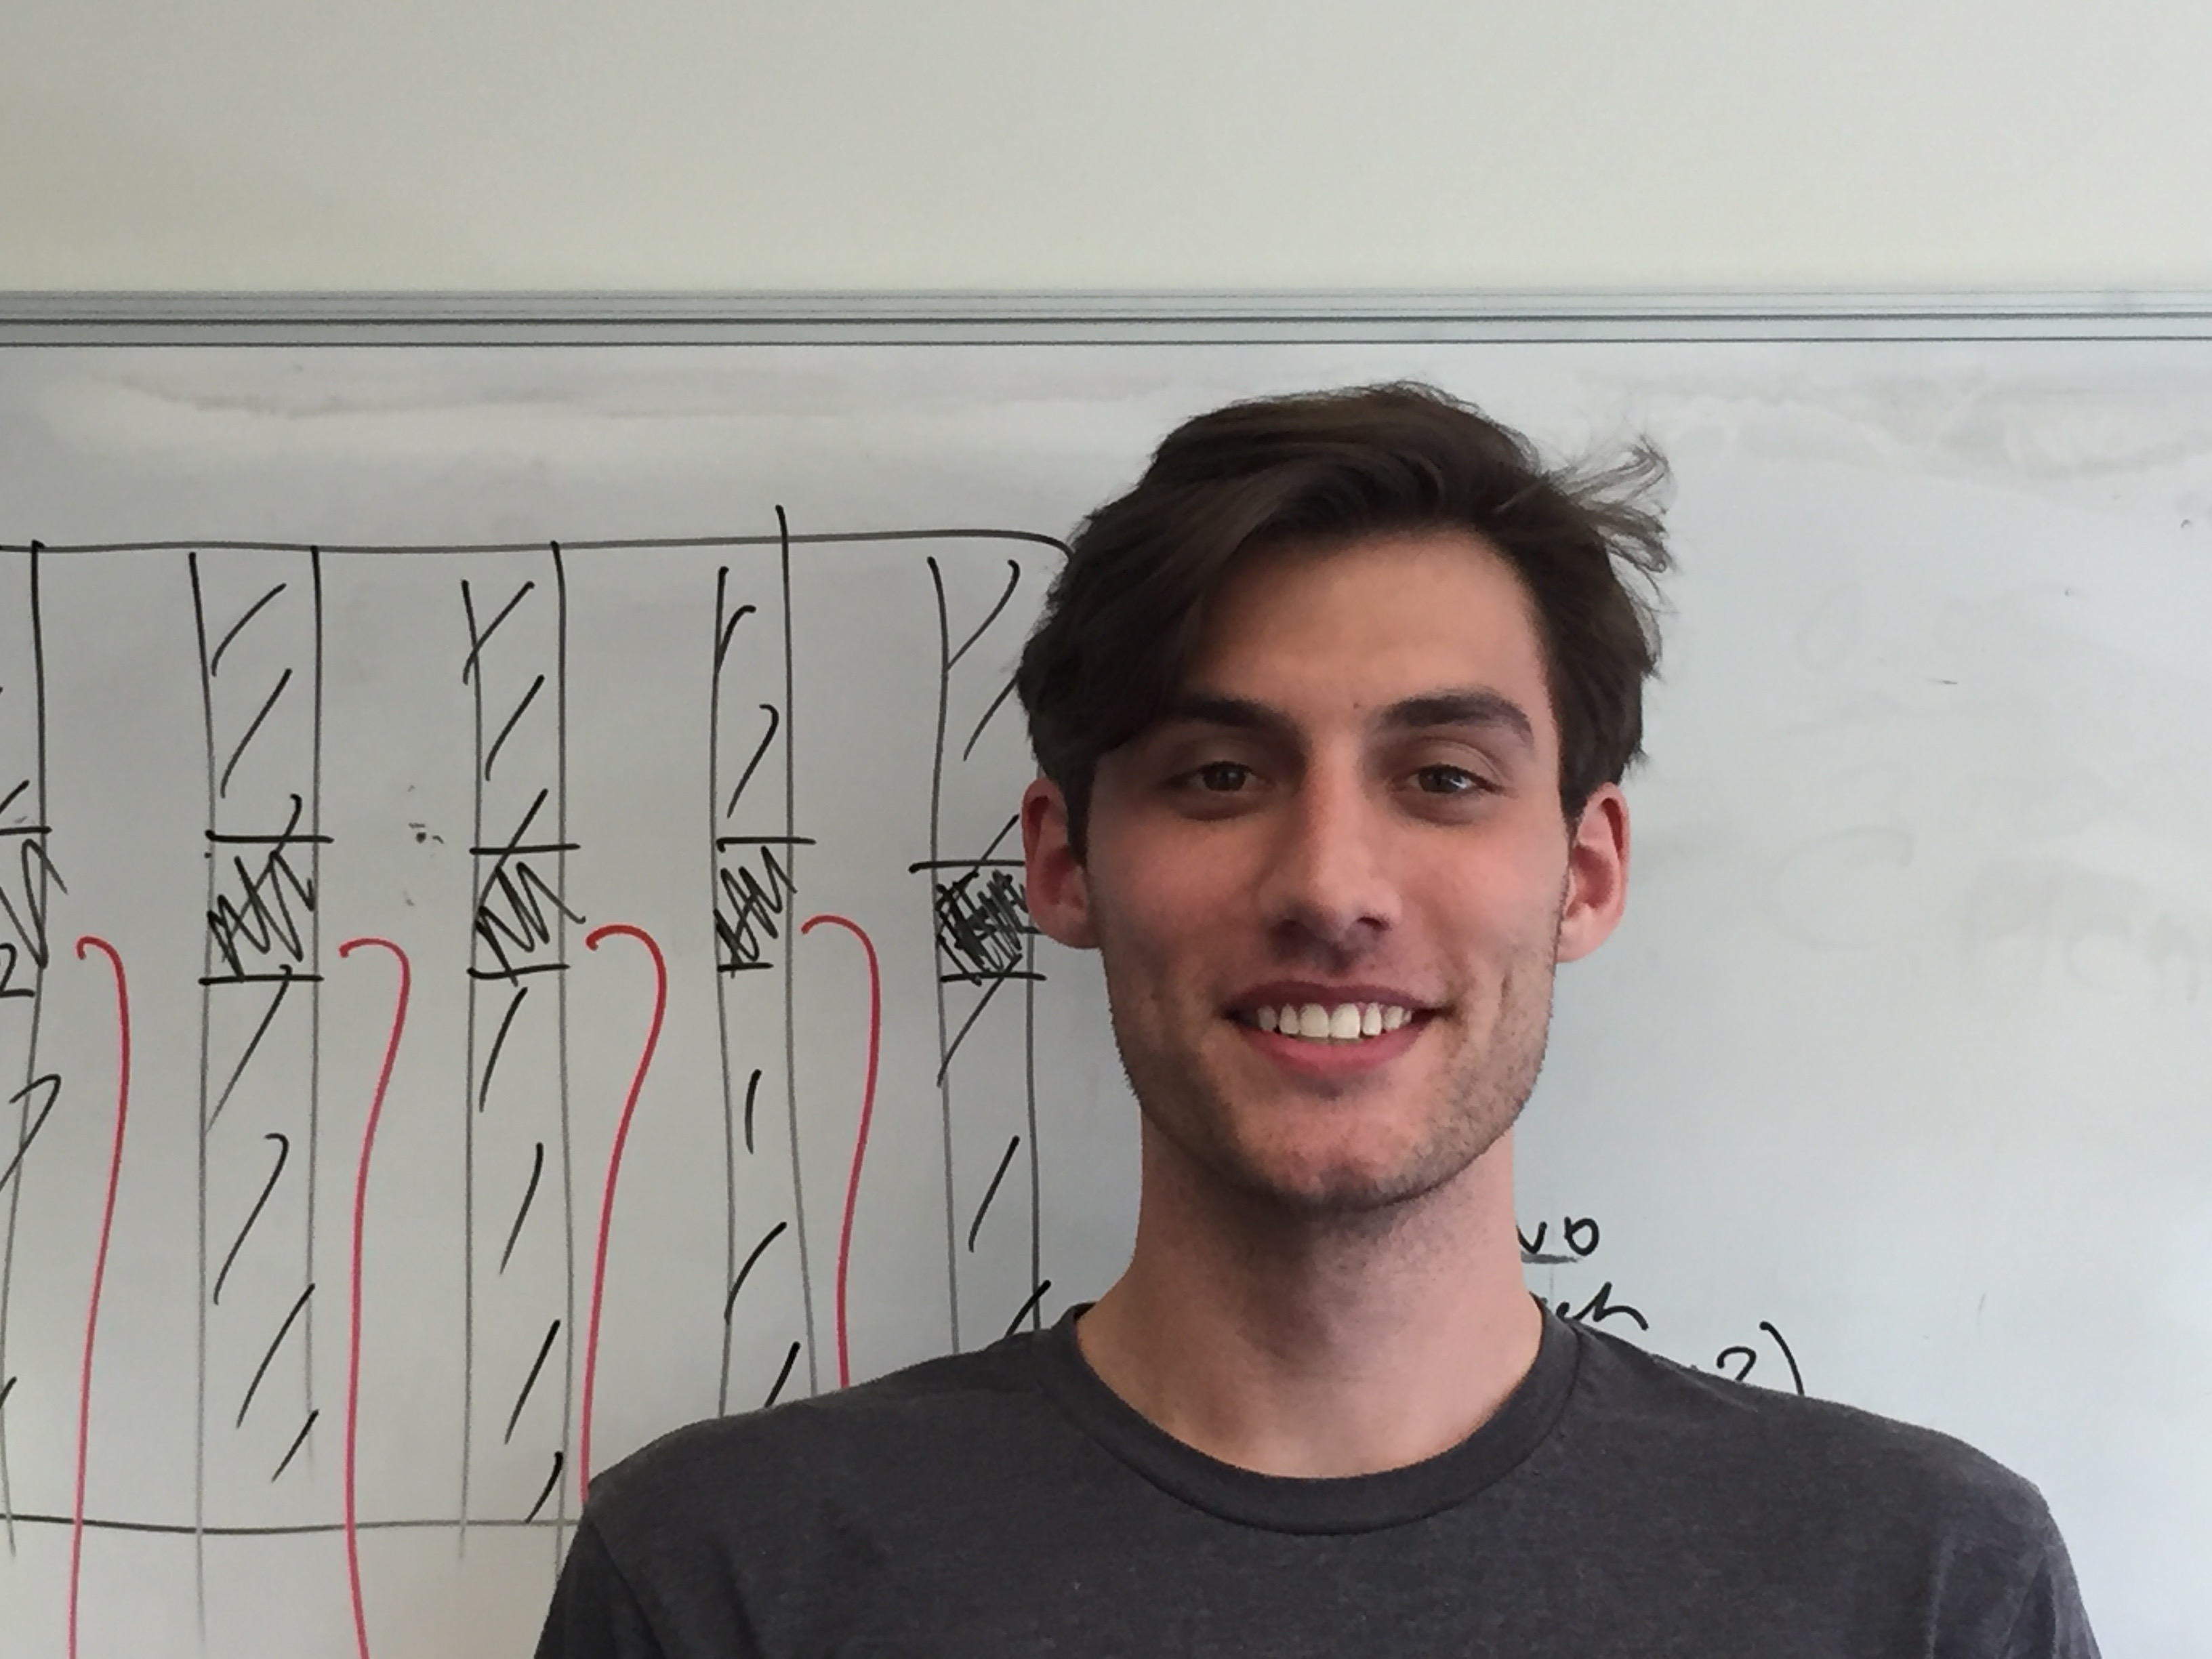
\includegraphics[width=\trainerIconWidth]{photos/al.jpg} &
    \textbf{Mr. Alastair Luddington}\newline
    Bioinformatician\newline
    Bioinformatics Hub\newline
    The University of Adelaide\newline
    South Australia\newline
    \mailto{alastair.luddington@adelaide.edu.au}\\
   \\  
\end{longtable}
\end{center}



%
% Workshop Preamble
%
%
% Start: General Information describing the workshop and the structure of the handouts
%
\newpage
\section{Welcome}
Thank you for your attendance \& welcome to the Introduction to NGS Data \& NGS Analytic Tools Workshop.
This is a free offering by the University of Adelaide, Bioinformatics Hub which is a centrally funded initiative from the Department of Vice-Chancellor (Research), with the aim of assisting \& enabling researchers in their work.
Training workshops \& seminars such as this one  are an important part of this initiative. \\

The Bioinformatics Hub itself has a web-page on the University website at \url{http://www.adelaide.edu.au/bioinformatics-hub/}.
To be kept up to date on upcoming events and workshops, please join the internal Bioinformatics mailing list on \url{http://list.adelaide.edu.au/mailman/listinfo/bioinfo}.
Also, please consider following the Bioinformatics Hub on Twitter as many handy hints are posted on this feed \url{https://twitter.com/UofABioinfoHub}.\\

Today's workshop has been prepared with generous technical support \& advice provided by Dr Nathan Watson-Haigh (\textit{ACPFG}), Dr Dan Kortschak (\textit{Adelaide University, Adelson Research Group}), Dr Zhipeng Qu (\textit{Adelaide University, Adelson Research Group}), Dr Mark Corbett (\textit{Robinson Institute}) \& Dr John Toubia (\textit{Adelaide Centre for Cancer Genomics}). 
The tutors today are Steve Pederson, Dr Hien To, Dr Jimmy Breen from the University of Adelaide, Bioinformatics Hub, \& Dr Terry Bertozzi (\textit{SA Museum \& Adelaide University, Adelson Research Group}). 
We hope it will be useful in enabling you to continue and to advance your research.\\

\section{Course Summary}
In today's workshop we will be introducing you to a small number of the basic tools required for NGS data handling, as well as giving you a basic familiarity with what the data actually looks like.
Whilst we will not be able to cover all of the rich \& diverse set of tools available, we hope to cover many of the key concepts \& questions to ask of your data, as well as give you an understanding of what information is actually in the data.\\

The majority of data handling and analysis required in the field of bioinformatics uses the \textit{command line}, alternatively known as the terminal or the \textit{bash shell}, so some useful tips for the command line will be included amongst the material.
Whilst most of the session will involve looking at individual files, in reality most of our analysis will be performed using some type of script to automate, \& easily reproduce an analysis. \\

Today's session is also intended to explore several tools in actual detail, rather than rush across the whole field.
There is large amount of information that we won't have time to discuss, but hopefully some important tools and thought processes will be covered \& enable you make better progress with your own datasets.\\

\section{Post Workshop}
The VMs which we work on today will remain active for week or so after the workshop, so feel free to continue exploring any sections that you weren't able to make it through.
We'd also encourage you to sign up for some of the high-traffic websites like \textit{BioStars} or \textit{SEQanswers} as these are a rich resource for your own problem solving.


\section{Document Structure}
We have provided you with a printed and an electronic copy of the workshop's hands-on tutorial documents.
We have done this for two reasons: 1) you will have something to take away with you at the 
end of the workshop, and 2) you can save time (mis)typing commands on the command line by using
copy-and-paste.

\emph{We advise you to use Acrobat Reader to view the PDF. This is because it properly supports some
features we have implemented to ensure that copy-and-paste of commands works as expected. This
includes the appropriate copy-and-paste of special characters like tilde and hyphens as well as
skipping line numbers for easy copy-and-past of whole code blocks.}\\
\\

\begin{warning}
While you could fly through the hands-on sessions doing copy-and-paste, you will learn more if you
use the time saved from not having to type all those commands, to understand what each command is
doing!
\end{warning}

The commands to enter at a terminal look something like this:
\begin{lstlisting}
tophat --solexa-quals -g 2 --library-type fr-unstranded -j annotation/Danio_rerio.Zv9.66.spliceSites -o tophat/ZV9_2cells genome/ZV9 data/2cells_1.fastq data/2cells_2.fastq
\end{lstlisting}  

The following styled code is not to be entered at a terminal, it is simply to show you the syntax of
the command. You must use your own judgement to substitute in the correct arguments, options,
filenames etc

\begin{lstlisting}[style=command_syntax]
tophat [options]* <index_base> <reads_1> <reads_2>
\end{lstlisting}

The following icons are used in the margin, throughout the documentation to help you navigate around
the document more easily:

% TODO limit the use of some icons throughout as some are clearly overused and confuse the eye
\hspace*{.2cm}\vcent{\includegraphics[height=1cm]{icons/info.png}} Important\\
\hspace*{.2cm}\vcent{\includegraphics[height=1cm]{icons/notes.png}} For reference\\
\hspace*{.2cm}\vcent{\includegraphics[height=1cm]{icons/steps.png}} Follow these steps\\
\hspace*{.2cm}\vcent{\includegraphics[height=1cm]{icons/questions.png}} Questions to answer\\
\hspace*{.2cm}\vcent{\includegraphics[height=1cm]{icons/warning.png}} Warning - STOP and read\\
\hspace*{.2cm}\vcent{\includegraphics[height=1cm]{icons/bonus1.png}} Bonus exercise for fast learners\\
\hspace*{.2cm}\vcent{\includegraphics[height=1cm]{icons/bonus2.png}} Advanced exercise for super-fast learners\\


\clearpage
%\section{Computer Setup}
\begin{information}
We will all be working on our own computers today, and will be accessing Virtual Machines running the Ubuntu operating system on \texttt{phoenix}, which is the University of Adelaide's High Performance Computing (HPC) system.
The software client \texttt{X2GO} which you will have already installed, enables us to access these machines in a familiar Desktop style, even though the majority of our time will be spent within the terminal. \\
\end{information}

You will have been allocated a VM with an associated IP address.
To connect to your VM, \textbf{please follow these instructions carefully}.
First, we need to create a session with the basic parameters
\begin{enumerate}
	\item Open X2GO
	\item Enter \textit{IntroductionToNGS} as the \textbf{Session Name}
	\item Enter your \textit{IP address} where it say \textbf{Host}
	\item Enter the word \textbf{hub} as the login. \textbf{This must be all lower-case}
	\item Select \textbf{XFCE} from the drop-down menu under \textbf{Session Type}
	\item Click OK
\end{enumerate}

Now we have created the session, it will appear in your X2Go on the right.
To log onto the VM, we simply click on the session, and enter the password \textbf{hub}.
\textbf{Click OK if you receive a message about a security key}.
If this process fails, please place the red post-it note on your monitor.\\

\textit{We advise maximising your X2Go window to replicate sitting at the VM as if it is your local machine.}

\begin{figure}[ht]
	\centering
	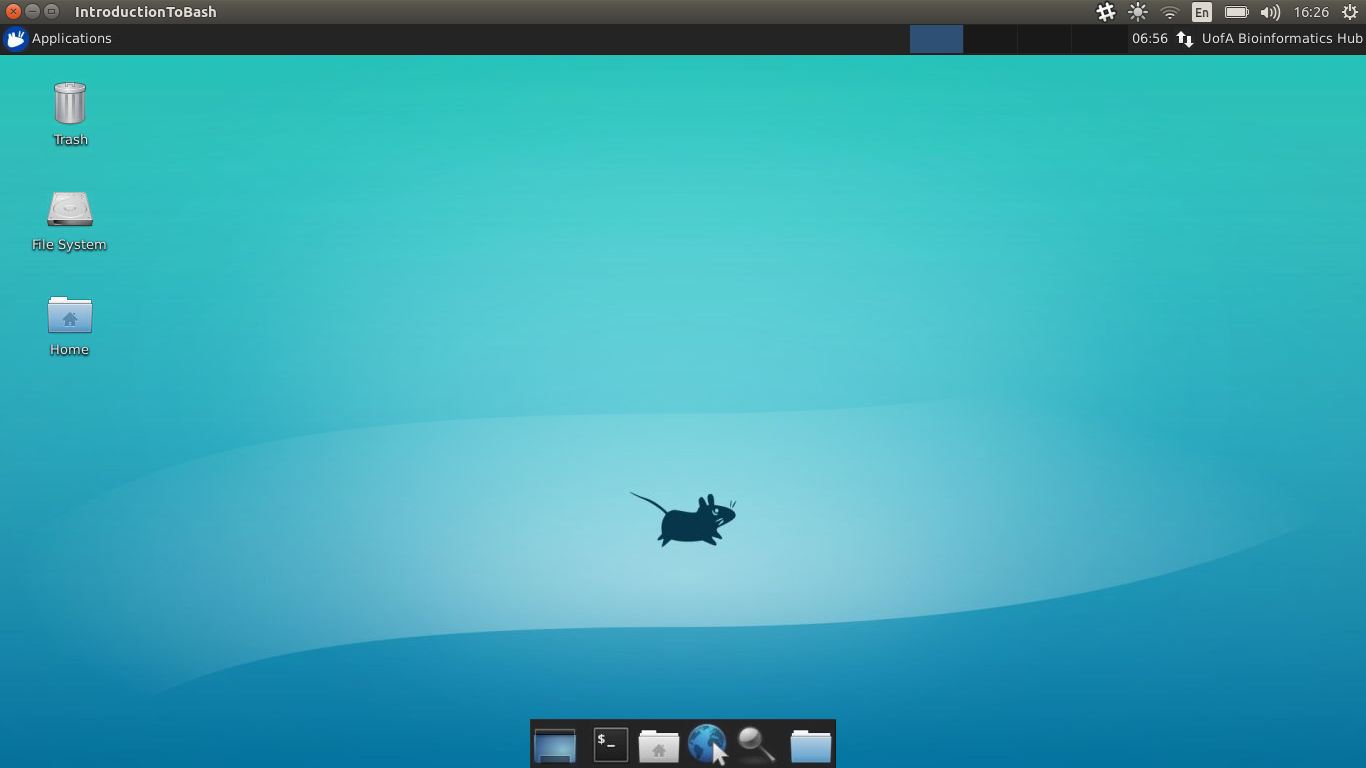
\includegraphics[width=0.9\linewidth]{images/xfceDesktop.png}
	\caption{The VM desktop after logon with X2GO}
\end{figure}


\section{The Ubuntu Desktop}
\begin{note}
Now that you are connected, you will notice we are in a standard graphical environment.
The default Desktop in Ubuntu is Unity, but what we are seeing is one of the many alternatives, known as XFCE.
We are using this as it is the most simple for remote connections.
As many of us are used to seeing, there are click-able icons on the desktop, and drop-down menus. \\

Although we won't be using them today, Ubuntu has an built-in Office Suite of
programs which you can access from the \textit{Applications \textgreater Office} menu item.
This is where links can be found to open Document Viewer (a .pdf viewer), Libre Office Calc (Excel-like), Libre Office Writer (Word-like) \& other standard members of Office Program Suites. \\

The main interface we will be using today is the \texttt{terminal}which can be accessed from the set of icons at the bottom of you screen.
\textbf{Firefox} can also be accessed from the terminal using the command \texttt{firefox \&},  by clicking the \texttt{Web Browser} icon, or from the drop-down menu in the top left under the group \textit{Internet}.

\end{note}


%
% Start of modules
% Switch chapter styling to module
%
\chapterstyle{module}


%
% End of modules
% Switch back to normal workshop chapter styling
%
\chapterstyle{workshop}

\chapter{Space for Personal Notes or Feedback}
\clearpage

%
% Some empty ruled comments pages
%
\myruledpage{0cm}{1cm}
\myruledpage{0cm}{1cm}
\myruledpage{0cm}{1cm}
\myruledpage{0cm}{1cm}

\end{document}
